\begin{document}
\title{Distributed Systems}
\subtitle{Computer Science Tripos, Part IB\\Michaelmas term 2020/21}
\author{Martin Kleppmann}
\institute{Department of Computer Science and Technology\\University of Cambridge}
\date{}
\maketitle

This is the title slide:

\begin{frame}
    \label{s:title}
    \begin{center}
        \textbf{\huge{\color{darkblue}{Distributed Systems}}} \\[2em]
        Martin Kleppmann (mk428@cam) \\[2em]
        University of Cambridge \\[0.5em]
        Computer Science Tripos, Part IB \\[0.5em]
        Michaelmas term 2020/21 \\[0.5em]
        \href{https://www.cl.cam.ac.uk/teaching/current/ConcDisSys/}{www.cl.cam.ac.uk/teaching/current/ConcDisSys/}
    \end{center}
\end{frame}

Followed by slide 2:

\begin{frame}
    \label{s:test}
    \frametitle{This is the frame title}
    Text in the frame

    partial synchrony
\end{frame}
\inlineslide{s:test}

\begin{frame}[plain]
    \label{s:snowball}
    \begin{center}
        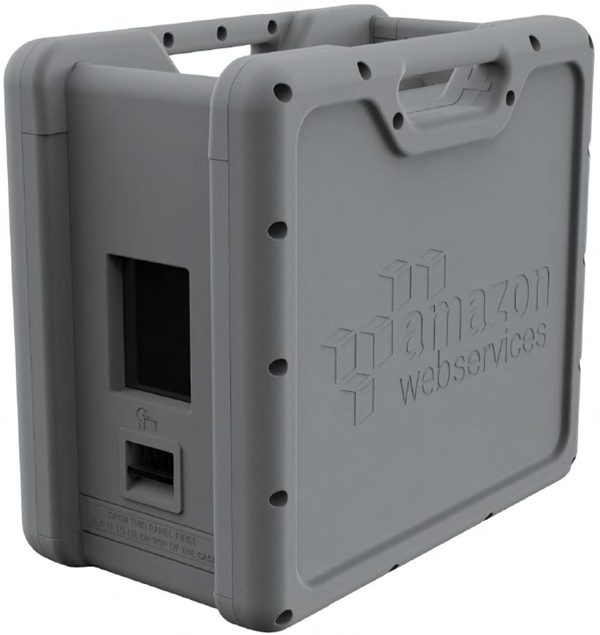
\includegraphics[height=7.5cm]{images/aws-snowball.png}\\[0.5em]
        \footnotesize{Source: \url{https://docs.aws.amazon.com/snowball/latest/ug/using-device.html}}
    \end{center}
\end{frame}
\inlineslide{s:snowball}

\section{Models of distributed systems}

Relationship between dist sys and networking: networking is how you get the bytes ``over the wire'' (or over the wireless network) to another machine; dist sys is what you do with the bytes once they get there.

The ``wire'' may actually be radio waves, lasers, hard drives in a van, or even a USB thumb drive in someone's pocket
% AWS Snowball: https://docs.aws.amazon.com/snowball/latest/ug/using-device.html

Fundamental abstraction: nodes (or processes); sending a message from one node to another.

``reliability'' of TCP; screenshots of network error + request timeout

Why distribute?
- Inherently distributed: communication, collaboration (Facebook, google docs).
- Scale, performance, fault tolerance

It's easy if you can do it on one machine! Don't distribute unless you have to. 

Distributed systems are fascinating because we have to work with partial knowledge and uncertain
truths. We never have certainty about the state of the system, because by the time we hear about
something, that state may already be outdated. In this way it resembles real life more than most of
computing! In real life you need to often make decisions with incomplete information.

Two generals problem, Byzantine generals problem
% two generals: https://link.springer.com/chapter/10.1007/3-540-08755-9_9

Calendar app supports offline reads and writes (short video in airplane mode).

\begin{itemize}
\item synchronous, partially synchronous~\cite{Dwork:1988dr}, and asynchronous model
\item crash-stop, crash-recovery, and arbitrary (Byzantine) faults
\item network may drop, duplicate, reorder packets (and even sniff and spoof?)
\end{itemize}

network message delay: synchronous, partially synchronous, asynchronous

network reliability: reliable, fair-loss, arbitrary. (fair-loss means non-zero probability of a
given message being delivered. links guarantee messages not created out of thin air -- see Cachin et al.
Arbitrary links need authentication.)

can we make a fair-loss link reliable? send acknowledgements and retransmit on timeout; deduplicate
on recipient side. however, in crash-recovery model, retry and deduplication state would be lost on
crash, so this needs to be maintained in stable storage.

Fundamental building blocks of distributed systems: replication and partitioning.

Replication example: two clients A and B, four servers. Server 1 receives only A's request,
server 2 receives A then B, server 3 receives B then A, and server 4 receives only B.
How do we ensure replicas become consistent with each other?

Use this as motivation for introducing causality and happens-before.
Show that physical timestamp ordering may  be inconsistent with causality.
Distinguish between A and B being concurrent, and A happening before B
(determining which one should overwrite the other).

ABD algorithm. Last writer wins. Linearizability.

notion of causality: taken from physics (relativity).
When a happened before b, that doesn't mean that a necessarily caused b; it just means that a \emph{might have} caused b.
For this reason, we sometimes say that the happens-before relationship encodes \emph{potential causality}.

However, when a and b happened independently (no message sent after a arrived before b, and no message sent after b arrived before a), we know that a \emph{cannot have caused} b and vice versa.

Hybrid Logical Clocks - Kulkarni et al, Logical physical clocks (OPODIS 2014) \url{https://doi.org/10.1007/978-3-319-14472-6_2}

Exercise. A relation R is a strict partial order if it is transitive ($\forall a,b,c.\; (a,b) \in R \wedge (b,c) \in R \Longrightarrow (a,c) \in R$) and irreflexive ($\nexists a.\; (a,a) \in R$). Show that the happens-before relation is a strict partial order.

Exercise. Show that for any two events $a$ and $b$, exactly one of the three following statements must be true: either $a \rightarrow b$, or $b \rightarrow a$, or $a \parallel b$.

% 1. Network communication basics: JSON, TCP, HTTP/REST, UDP. Hands-on: using things like tcpdump?
% 2. Faults and failures
% 3. Architectures: client-server, local networks (multicast), peer-to-peer (distributed hash tables, NAT traversal)
% 4. Programming models: services, RPC, message brokers, actors, map-reduce, stream processing, tuple spaces?
% 5. Replication
% 6. Consensus
% 7. Convergence
% 8. Time and clocks
% 9. Security (e.g. TLS), byzantine fault tolerance, and blockchains

% Live demo of RESTful API with Dropwizard, curl, browser access

% State machine replication

% "causality is reachability in spacetime"
% https://twitter.com/palvaro/status/1233208997257170944

% message loss -> retry; duplicates -> detect and suppress duplicates / idempotence
% idempotence: f(f(x)) = f(x)
% incrementing number of likes on a post: not idempotent
% adding current user to the set of users who have liked a post: idempotent
% what state must a recipient maintain in order to eliminate duplicates?
% the entire message? a unique message ID? a sequence number? (what assumptions does this require making about the sender?)

% MIT graduate dist-sys course https://pdos.csail.mit.edu/6.824/schedule.html
% Raft animations: http://thesecretlivesofdata.com/raft/

\bibliographystyle{plainurl}
\bibliography{references}{}
\end{document}
